\newgeometry{left=4.5cm, right=4.5cm,bottom=4cm, top=4cm}

\chapter{The Higgs Bosons and the MSSM} \label{chap:theory}

 \vspace{2cm}

This chapter  introduces the theoretical concepts relevant for the experimental search presented in this thesis.
A brief overview of the Standard Model of particle physics is given in Section~\ref{sec:SM} based on Reference~\cite{Altarelli}. 
Among all the extension of the Standard Model, the Minimal Supersymmetric 
extension (MSSM) is  theoretically favoured  as one of the most predictive
scenarios beyond the Standard Model. The MSSM is introduced in Section~\ref{sec:MSSM} with an enphasis on the Higgs boson physics, based on 
References~\cite{SusyPrimer,Djuadi}.
Finally, a review of phenomenological aspects related to the MSSM Higgs bosons is given 
in Section~\ref{sec:pheno}, based on Reference~\cite{LHCxsec}.
%In section... introduction is given based on~\cite{Altarelli}, 
%This chapter is devoted to introduce the the Minimal Supersymmetric 
%extension of the Standard Model (MSSM) whit focus on  its Higgs sector.
%In section... introduction is given based on~\cite{Altarelli}, 

\restoregeometry

\clearpage

\section{The Standard Model of Particle Physics} \label{sec:SM}
\subsection{Introduction}
A detailed description of the Standard Model (SM) of particle physics may be found in Reference~\cite{Peskin}, only a brief overview is
given below.

The SM of particle physics is a theory aimed to describe and quantitatively predict
the phenomenology of fundamental particle interactions. At the quantum  level the spectrum of all interactions between matter and 
radiation can be understood in terms of three fundamental forces: the strong, the electromagnetic
and the weak forces. These interactions are described by a local relativistic quantum field theory, where 
a field with suitable transformation properties under the Lorentz group is associated to each particle.
The theory is based on the principle of gauge invariance, i.e. invariance under  symmetry  transformations    
that operate on basic internal degrees of freedom and depend on the space-time coordinate.
The gravitational force is negligible in atomic and nuclear physics, since the
quantum effects of gravity are expected only at very high energies corresponding to the Planck mass $E \sim M_{Planck} c^2 \sim 10^{19}$~GeV.

The SM is a gauge field theory based on the symmetry group $SU(3)_c \otimes SU(2)_L \otimes U(1)_Y$. The group has $8+3+1=12$
generators with a non trivial commutator algebra. The electromagnetic and weak interactions~\cite{EW1,EW2,EW3}  are described  by the 
$SU(2)_L \otimes U(1)_Y$ symmetry group, while the $ SU(3)_c$ is the colour group of the theory of strong interactions (QCD)~\cite{qcd1}.
A vector boson is associated to each generator of the symmetry group, which acts as a mediator of the corresponding interaction.
Eight gluons are associated to the $ SU(3)_c$ colour generators, while  four gauge bosons $W^{\pm}$,
$Z^0$ and $\gamma$ are associated to the generators of $SU(2)_L \otimes U(1)_Y$. 
The gluons and the photon are massless, while the remaning bosons have mass  since the symmetry induced by the other three generators is
spontaneously broken. In the SM the spontaneous symmetry breaking is realised by the Higgs mechanism~\cite{ENGLERT,HIGGS,HIGGS2,HIGGS3,kibble}.
The Higgs boson acts as mediator of a new class of interaction whose stregth, at tree level, increases proportionally to the particle masses.

The fermionic matter fields of the SM are quarks and leptons. 
Quarks  are subject to all SM interactions, each quark type  is a colour triplet and carries 
electroweak charges, in particular the electric charge for up-type quarks is $+2/3$ and $-1/3$
for down-type quarks.  Leptons are colourless
but have electroweak charges, the leptons  $e$, $\mu$ and $\tau$ carry an  electric charge of $-1$,
while neutrinos $\nu_e$, $\nu_{\mu}$ and $\nu_{\tau}$ are electrically neutral. Opposite sign charges
are intended for respective anti-particle.
Quarks and leptons are grouped in three  ``generations'' with equal quantum numbers but with different masses.

%\subsection{The Higgs Mechanism in the SM}


\subsection{Precision Tests and Limitations of the SM}

The Standard Model has been successfully tested in a vast number of experiments over a wide range of energies during the last decades.
Precision tests of the electroweak theory performed at LEP, SLC and the Tevatron~\cite{smtest} have 
confirmed that the couplings of quark and leptons to the weak gauge bosons $W^{\pm}$  and $Z$ fully agree 
with the predictions from the gauge symmetry. Due to the experimental accuracy of a few per-mille, not only the tree level
calculations, but also the impact of quantum corrections have
been verified. Several other experimental results~\cite{pdg}
including rare decays of hadrons provide additional tests of the Standard Model at low energies. 
The recent discovery at the LHC of a Higgs boson   with a mass $m_H \sim 126$~GeV \cite{AHiggsO,CHiggsO} 
is also another success of the SM, the measured mass is in agreement with value expected from a 
global fit of electroweak observables~\cite{gfitter}, the spin and couplings properties of this new boson are also 
in good agreement with SM predictions for such mass.

%Among all the parameters of the Standard Model only few of them presents 
Tension between the SM prediction and  experimental data is observed for only a few observables. 
The most significant discrepancies, which are slightly above three standard deviations, are observed for the anomalous magnetic moment 
of the muon $a_{\mu}$~\cite{gminus2} and for the forward-backward asymmetry in the top quark production $A_{FB}^{\ttbar}$~\cite{FBasymmetry}.   


Inspite of this success, the Standard Model is conceptually unsatisfactory due to a number of deficiencies and is
widely believed to be an effective theory valid only at presently accessible energies. In addition to the fact that 
the SM does not  include the  gravitational force, it does not explain the pattern of fermion masses and in its simplest 
version does not include neutrino masses, the theory has at least three other conceptual problems indicating the need 
for new physics beyond the Standard Model (BSM):
%\begin{itemize}
%\item
\paragraph{Hierarchy Problem} The radiative corrections to the Higgs boson mass introduce quadratic divergences of the order  
	of the cut-off energy scale $\Lambda$, above which the theory is considered to be invalid and new physics 
	is expected to appear~\cite{Lambda}. If the cut-off scale is chosen to be $\sim M_{Planck}$, then a fine tuning 
	between the tree-level and higher order calculations is needed with an unnaturally high precision of $\mathcal{O}(10^{-30})$
	to cancel these divergences  and result in a  Higgs boson mass of the order of the electroweak breaking scale, $M_{EW}\sim\mathcal{O}(100\,GeV)$.
	The SM provides no satisfactory answere to the question on  how these cancellations can occur and why $\Lambda >> M_{EW}$. These problems are
	referred to as the fine-tuning and hierarchy problem~\cite{Hierarchy1,Hierarchy2,Hierarchy3}.
	%Supersymmetry was first introduced to answer this question, indeed, the new symmetry prevents the Higgs boson mass to acquire very large 
	%radiative corrections, the quadratic divergent loop of the SM particles are exactly cancelled by the loop contribution 
	%of the corresponding partners, solving in this way the hierarchy problem~\cite{Djuadi5}.

%\item
\paragraph{Dark Matter}   The SM does not contain a particle candidate which would explain the large contribution 
	of non-barionic, non-luminous matter (so-called dark matter) to the density of the universe~\cite{darkmatter1,darkmatter2,darkmatter3}. 
	To be a dark matter candidate a particle should be stable, massive and should be weakly interacting with the known SM particles. 
	%Supersymmetry models,  provided with R-parity conservation,
	%provides a natural candidate for Dark Matter, which would be then the lightest SUSY particle which cannot further decay.

%\item 
\paragraph{Unification Problem}	Another unsatisfactory aspect of the SM is that the electroweak and strong interactions cannot be unified, i.e.
	their couplings do not converge to the same value at high energies. Motivated by the successful unification of electromagnetic and weak
	interaction, the existence of Grand Unified Theory (GUT) has been 
	suggested~\cite{GUT1,GUT2}, which predicts the unification of all the three gauge coupling strengths at the GUT energy scale,
	$\Lambda_{GUT} \simeq 10^{16}$~GeV and describes the three forces within a single gauge group with just one coupling constant.
	%The particle spectrum in SUSY, instead, contributes to the renormalisation group evolution of the three gauge couplings constants and 
	%favours them to meet at energies around $10^{16}$ GeV~\cite{djuadi4}. 

%\end{itemize}
\vspace{0.5cm}
Among many possible extension of the SM, supersymmetry is one of the  theoretically strongly favoured scenarios as 
as it provides elegant solutions to the above problems. 
As discussed in Section~\ref{sec:MSSM}, it gives a natural answer to the hierarchy problem, provides a suitable dark matter candidate 
and predicts unification of the three gauge couplings at the GUT energy scale.


% the conceptual situation with the
%standard model is unsatisfactory for quite a few deficiencies:
%– the smallness of the electroweak scale v ∼ 246GeV << MPl (the ‘hierarchy problem’);
%– the large number of free parameters (gauge couplings,
%vacuum expectation value, MH, fermion masses,
%CKM matrix elements), which are not predicted but have
%to be taken from experiments;
%– the pattern that occurs in the arrangement of the
%fermion masses;
%– the missing way to connect to gravity.
%
%-Dark matter
%
%-neutrino masses

 
\section{The Minimal Supersymmetric Standard Model}\label{sec:MSSM}
\subsection{Introduction to the MSSM}
Supersymmetry (SUSY)~\cite{Susy1,Susy2,Susy3} was first introduced as a natural  solution to the hierarchy problem by means of
a new symmetry that relates bosons to fermions.
The SUSY generators $\mathcal{Q}$ transform fermions into bosons and vice versa:
\begin{equation}
\mathcal{Q}|\text{Fermion}\rangle = |\text{Boson}\rangle, ~ ~ ~ \mathcal{Q}|\text{Boson}\rangle = |\text{Fermion}\rangle\,.
\end{equation}
In a supersymmetric extension of the SM  each of the known fundamental particles 
is in either a chiral or gauge \emph{supermultiplet} and must have a superpartner with spin differing by 1/2 unit.
SUSY naturally solves the hierarchy problem since the quadratically divergent loop contributions to the Higgs mass from the SM 
particles are cancelled out by the loop contributions from the corresponding superpartners. 
The quarks and leptons  superpartners are named by adding an ``s'', standing for scalar, as prefix to the name of the corresponding
SM particle.
Accordingly, the gauge bosons related to the generator of the group $SU(3)_c \otimes SU(2)_L \otimes U(1)_Y$ should also have a spin 1/2 partner,
which is named adding ``ino'' as suffix to the SM name. The symbol of superpartners is defined by adding a ($\tilde{ ~ }$) to the SM symbol.
The SUSY particles share the same couplings with their SM partner, since the left-handed and right-handed components of fermions 
transform differently under gauge transformations also their superpartner inherit this feature.

The  Minimal Supersymmetric extension of the Standard Model  (MSSM)~\cite{MSSM1,MSSM2,MSSM3,MSSM4,MSSM5,MSSM6}, 
is defined by requiring the minimal gauge group (i.e., the one of the SM)
and the minimal particle content: three generation of fermions (without right-handed neutrinos), gauge bosons and two Higgs doublet, 
each with its own superpartner. The  chiral and gauge supermultiplets of the MSSM 
are listed in Tables~\ref{tab:chiralsup} and~\ref{tab:gaugesup}, respectively.
Among the gauge eigenstates listed in these tables, the superpartners of the Higgs bosons, the \emph{higgsinos}, mix with the \emph{wino}
and \emph{bino} to produce the mass eigenstates: two charginos $\chi_{1,2}^\pm$ and four neutralinos $\chi_{1,2,3,4}^0$.
\begin{table}
\begin{center}
\renewcommand{\arraystretch}{1.5}
\begin{tabular}{c|ccc}
\hline%\noalign{\smallskip}
Names 			&Supermultiplets	&	Spin 1/2  		& Spin 0 \\%[0.1cm]
\hline%\noalign{\smallskip}		
quark, squarks		& $Q$ 			&	$(u_L ~ d_L)$		& $( \tilde{u}_L ~ \tilde{d}_L)$ \\%[0.1cm]
($\times$ 3 families)	& $\bar{u}$		& 	$u_R^{\dagger}$ 	& $\tilde{u}_R^*$ \\%[0.1cm]
			& $\bar{d}$		& 	$d_R^{\dagger}$ 	& $\tilde{d}_R^*$ \\%[0.1cm]
\hline%\noalign{\smallskip}
leptons, sleptons	& $L$			&   	$(\nu ~ e_L)$ 		&  $( \tilde{\nu} ~ \tilde{e}_L)$\\%[0.1cm]
($\times$ 3 families)	& $\bar{e}$		&	$e_R^{\dagger}$         & $\tilde{e}_R^*$ \\%[0.1cm]
\hline%\noalign{\smallskip}
higgsinos, Higgs	& $H_1$			&	$( \tilde{H}_1^0 ~ \tilde{H}_1^-)$  &	$( H_1^0 ~ H_1^-)$ \\%[0.1cm]	 
			& $H_1$			&	$( \tilde{H}_2^+ ~ \tilde{H}_2^0)$  &	$( H_2^+ ~ H_2^0)$ \\%[0.1cm]	 
\hline
\end{tabular}
\caption{The chiral supermultiplets in the Minimal Supersymmetric Standard Model. The spin-0 fields are complex scalars
	and the spin-1/2 are left-handed two-component Weyl fermions. Based on Ref.~\cite{SusyPrimer}.}
\label{tab:chiralsup}
\end{center}
\end{table}

\begin{table}
\begin{center}
\renewcommand{\arraystretch}{1.5}
\begin{tabular}{c|ccc}
Names			&Supermultiplets& Spin 1 		&	Spin 1/2 \\
\hline
gluons, gluinos		&$G_a$ (a =1,...,8)	& $g$			& $\tilde{g}$	\\
W bosons, winos		& $W_a$ (a=1,...,3)	& $W^{\pm}$ $W^0$	& $\tilde{W}^{\pm}$ $\tilde{W}^0$ \\
B boson, bino		&$B$			& $B^0$			& $\tilde{B}^0$ \\
\hline
\end{tabular}
\caption{ The gauge supermultiplets in the Minimal Supersymmetric Standard Model.Based on Ref.~\cite{SusyPrimer}.}
\label{tab:gaugesup}
\end{center}
\end{table}

\subsubsection{$R$-parity conservation}
The MSSM requires a discrete and multiplicative symmetry called $R$-parity~\cite{Susy3}. This symmetry ensures the barion and lepton number 
conservation and it is defined as follows:
\begin{equation}
R_p = (-1)^{2s+3B=L}
\end{equation}
where $L$ and $B$ are lepton and barion numbers and $s$ stands for the spin quantum number. The R-parity quantum number has a value of $+1$ for ordinary
SM particles and $-1$ for their superpartners. This symmetry was originally introduced as a simple solution to protect against the instability of the proton.
Lepton and barion number violation leads, in many cases, 
to an unstable proton with a life-time shorter than the experimental lower bound. The $R$-parity conservation has also other important 
phenomenological consequences: SUSY particles are always produced in pairs and decay always into an odd number of SUSY particles.
Furthermore, the lightest SUSY particle, often chosen to be one of the neutralinos, is stable and therefore provides a suitable 
candidate for the dark matter.


\subsubsection{The Soft SUSY Breaking}
If supersymmetry is an exact symmetry of nature, the SM particles and their corresponding superpartners should have the same mass 
and quantum numbers, except for the spin. However, the SUSY particle spectrum  has not yet been observed, suggesting that  these particles,
if they exist,  should be heavier than their SM superpartners. 
To achieve such SUSY-breaking without reintroducing the quadratic divergences to the Higgs mass value, a so called ``soft-SUSY-breaking''
term is introduced to the SUSY Lagrangian~\cite{softerm1,softerm2}. This term explicitly breaks SUSY by introducing the mass terms for the 
Higgs bosons, gauginos and
sfermions, as well as  trilinear coupling terms between sfermions and Higgs bosons. In general, if intergenerational mixing and 
complex phases are allowed, the soft-SUSY-breaking terms will introduce a very large number of unknown parameters $\mathcal{O}(100)$~\cite{softerm3}.
However, in absence of these phases and  mixings, and if the soft terms obey  a set of boundary conditions~\cite{softerm1,softerm2}, 
only a few new parameters are introduced ($\mathcal{O}(10)$).




\subsection{The Higgs Sector in the MSSM }\label{sec:hsector}
In the MSSM two doublets of complex scalar fields of opposite hypercharge are required to break the electroweak symmetry. 
This requirement is necessary to separately generate the masses of isospin up-type fermion and down-type fermions~\cite{Susy2,Higgsm1,Higgsm2}
and to cancel chiral anomalies that otherwise would spoil the renormalizability of the theory~\cite{Higgsm3}. The two Higgs doublets  are:
\begin{equation}
H_1 = \binom{H_1^0}{H_1^-} ~ ~ \text{with } Y_{H_1} = -1, \quad \text{and} \quad H_2 = \binom{H_2^+}{H_2^0} ~ ~ \text{with } Y_{H_2} = +1 \,. 
\end{equation}
In analogy with the SM, a similar Higgs mechanism is employed in the MSSM~\cite{MSSM1,Higgsm4}  requiring that the minimum 
of the Higgs potential breaks the $SU(2)_L \otimes U(1)_Y$ symmetry while preserving the electromagnetic symmetry $U(1)_Q$.
The neutral components of the 
two Higgs field acquire vacuum expectation values:
\begin{equation}
\langle H_1^0 \rangle = \frac{v_1}{\sqrt{2}}, \quad \text{and} \quad  \langle H_2^0 \rangle = \frac{v_2}{\sqrt{2}}\,.
\end{equation}
Three of the original eight degrees of freedom of the scalar fields are absorbed by the $W^{\pm}$ and $Z$ bosons, which acquire
their longitudinal polarisations and masses. The remaining degrees of freedom correspond to five physical Higgs bosons: two neutral CP-even 
bosons $h$ and $H$, 
a neutral CP-odd boson $A$ and a pair of charged bosons $H^{\pm}$. 
The MSSM Higgs sector is described by six parameters: the Higgs bosons masses $M_h$, $M_H$, $M_A$, $M_{H^\pm}$,
the mixing angle $\alpha$ in the neutral CP-even sector  and the ratio between the two vacuum expectation values $\tan \beta = v_1/v_2\,$.
At tree level,  only two of these parameters  are  independent, commonly chosen to be  $\tan \beta$ and $M_A$. 
The supersymmetric structure of the theory imposes a strong hierarchical structure of the Higgs boson mass spectrum:  
the $h$ boson is the lightest  and at tree level is found that  $M_h < M_Z$, while $M_A < M_H$ and $M_{H^\pm}^2 = M_A^2 M_W^2$. Furthermore, the 
following relation holds between the mixing angles:
\begin{equation}\label{eq:mixing}
\cos^2(\beta - \alpha) = \frac{M_h^2 (M_Z^2 - M_h^2)}{M_A^2 (M_H^2 - M_h^2)}
\end{equation}
These relations are broken by large radiative corrections to the Higgs bosons 
masses~\cite{Higgsm5}, which among others raise the threshold of the  $h$ boson mass from  $M_Z$ to $\mh \apprle 140$ GeV.
Additionally the GUT assumptions restrict the $\tan\beta$ value to the range  $1 \apprle \tan \beta \apprle m_t/m_b$ ~\cite{Higgsm6}.


\section{Phenomenology of the Neutral MSSM Higgs Bosons}\label{sec:pheno}

\subsection{Couplings of the MSSM Higgs Bosons to SM Particles}\label{sec:couplings}
The phenomenology of the MSSM Higgs bosons depends on their couplings to the standard model and supersymmetric particles. 
A short overview of the former is given below, based on the Ref.~\cite{Djuadi}. Supersymmetric particles are assumed
to be heavy enough to prevent for direct Higgs bosons decays into these particles. 

%The Feynman diagram for 
The possible couplings between the MSSM Higgs bosons and vector bosons are shown in Figure~\ref{fig:couplings}, these are 
%are shown in Figure~\ref{fig:couplings}, where is possible to identify 
the three-linear couplings $V_{\mu}V_{\nu}H_i$ of one  Higgs boson to two gauge bosons and $V_{\mu}H_{i}H_j$ of one gauge boson to two Higgs bosons,
as well as the quartic couplings between two Higgs bosons and two gauge bosons $V_{\mu}V_{\nu}H_iH_j$.
\begin{figure}[tp]
     \begin{center}
     \subfigure[]{		
            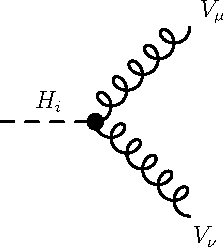
\includegraphics[height=3cm]{feyn_diagrams/diagrams/couplingHVV.pdf}
     }	\hspace{0.5cm}
     \subfigure[]{		
            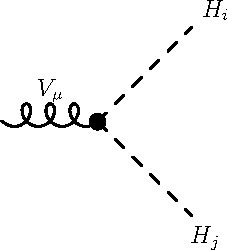
\includegraphics[height=3cm]{feyn_diagrams/diagrams/couplingVHH.pdf}
     }	\hspace{0.5cm}
     \subfigure[]{		
            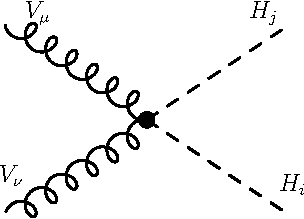
\includegraphics[height=3cm]{feyn_diagrams/diagrams/couplingVVHH.pdf}
     }
     \end{center}
   \label{fig:couplings}
    \caption{Feynman diagrams for the couplings between one Higgs boson and two gauge bosons (a), two Higgs bosons and one gauge boson (b)
		and two Higgs bosons and two gauge bosons (c)~\cite{Djuadi}. }
\end{figure}
Among them, the most relevant coupling for MSSM Higgs phenomenology is  the trilinear coupling $V_{\mu}V_{\nu}H_i$.
Since the photon is massless, there are no Higgs-$\gamma\gamma$ and Higgs-$Z\gamma$ couplings at tree level. CP-invariance also forbids $WWA$, $ZZA$
and $WZH^{\pm}$ couplings. Then, for the $V_{\mu}V_{\nu}H_i$ coupling only the following terms remain:
\begin{align} 
Z_{\mu}Z_{\nu} h ~ :  ~ & ig_z M_Z \sin(\beta -\alpha) g_{\mu\nu},  &  Z_{\mu}Z_{\nu} H ~ : ~  ~    & ig_z M_Z \cos(\beta -\alpha) g_{\mu\nu} \label{eq:couplings1} \\ 
W_{\mu}^+W_{\nu}^- h ~: ~&  ig_w M_W \sin(\beta -\alpha) g_{\mu\nu},  &  W_{\mu}^+W_{\nu}^- H ~ : ~ ~ & ig_w M_W \cos(\beta -\alpha) g_{\mu\nu} \label{eq:couplings2} 
\end{align}
The coupling strenght of the neutral CP-even Higgs bosons $h$ and $H$ to a pair of vector bosons are proportional to $\sin(\beta -\alpha)$ and $\cos(\beta -\alpha)$
respectively, where $\cos(\beta -\alpha)$ is fixed at tree level following equation~\eqref{eq:mixing}. An interesting phenomenological consequence is
that, with $G_{VVh}$ and $G_{VVH}$ being the coupling between two generic vector bosons and one of the two neutral CP-even Higgs bosons the following equation holds:
\begin{equation}\label{eq:couplingSM}
G^2_{VVh} +G^2_{VVH} = g^2_{VVH_{SM} }\,, 
\end{equation}
where $g^2_{VVH_{SM}}$ is the SM Higgs boson coupling. 
The equations~\eqref{eq:couplings1}-\eqref{eq:couplingSM} imply that the couplings of $h$ ($H$) to  vector bosons 
increase (decrease) with $\tan\beta$. For relatively large value\footnote{For most scenarios this is valid for  $\tan\beta \apprge 10$ 
 and large range of $m_A$.} 
of $\tan\beta$, $h$ has SM-like couplings to vector bosons while
 $H$  decouples from them. For an overview of all  other
coupling properties  between vector bosons and Higgs bosons, charged Higgs bosons, trilinear and quartic couplings among Higgs bosons and couplings 
to SUSY particles refer to~\cite{Djuadi}.

The coupling of the MSSM Higgs bosons to the isospin up-type ($u$), and down-type ($d$) fermions also depend on $\tan\beta$ and may be written
as follows:
\begin{small}
\begin{align*}
G_{huu} ~\propto ~ & m_u [\sin(\beta - \alpha)  + \cot\beta \cos(\beta - \alpha)], & G_{hdd} ~\propto ~ & m_u [\sin(\beta - \alpha)  - \tan\beta \cos(\beta - \alpha)]\\
G_{Huu} ~\propto ~& m_u [\cos(\beta - \alpha)  - \cot\beta \sin(\beta - \alpha)], & G_{Hdd} ~\propto~  & m_d [\cos(\beta - \alpha)  + \tan\beta \sin(\beta - \alpha)]\\
G_{Auu} ~ \propto ~ & m_u  \cot\beta, & G_{Add} ~ \propto ~ & m_d \tan\beta 
\end{align*} 
\end{small}
The couplings to down-type (up-type) fermions of either the $h$ or $H$ boson is enhanced (suppressed) by a factor $\tan\beta$, depending
on the magnitude of $\cos(\beta - \alpha)$ or $\sin(\beta - \alpha)$, while the coupling of $A$ boson to down-type (up-type) fermions are directly 
enhanced (suppressed) by $\tan\beta$.


\subsection{MSSM Benchmark Scenarios} \label{sec:benchmark}
At tree level, the MSSM  Higgs boson masses, decay branching fractions and production cross sections are all determined by two independent parameters,
conventionally chosen to be $M_A$ and $\tan\beta$. As pointed out in Section~\ref{sec:hsector}, 
the MSSM Higgs bosons masses are strongly affected by radiative corrections and the prediction of physics observables becomes 
dependent on additional MSSM parameters~\cite{Higgsm5}.
The main corrections arise from the top-stop (s)quark sector and for large $\tan\beta$ values also the bottom-sbottom (s)quark sector becomes increasingly 
important. Furthermore, the corrections are dependent on the SUSY-breaking scale $M_{SUSY}$, the trilinear Higgs-stop and  
Higgs-sbottom Yukawa couplings, as well as the electroweak gaugino and gluino mass parameters.

Due to the large number of free parameters, a complete scan of the MSSM parameter space is impractical for experimental searches and phenomenological
studies. To cope with this difficulty, several benchmark scenarios have been proposed~\cite{LHCxsec,mhmax2} which fix the 
values of the SUSY parametrs (entering the predictions via radiative corrections)
to particular benchmark values exhibiting interesting features of the MSSM Higgs phenomenology. The parameters 
$M_A$ and $\tan\beta$ are left free to vary and the results are usually presented in the $M_A-\tan\beta$ plane.

The $m_h^{max}$ benchmark scenario~\cite{MSSMmhmax} was  frequently  used  in the past searches for neutral MSSM Higgs bosons performed
at LEP, Tevatron and LHC~\cite{LEPLimits,TevatronLimits1,CMSLimit,ATLASLimit}. 
In this benchmark scenario, the MSSM parameters  are fixed such that the mass of the light CP-even Higgs boson $M_h$ 
assumes its maximal value as a function of $M_A$ and $\tan\beta$. The $m_h^{max}$ scenario allows to set conservative 
lower bounds on the values of $M_A$, $M_H^{\pm}$ and $\tan\beta$~\cite{mhmax2}. However, given the recent discovery of a Higgs
boson with mass of about $125$~GeV, this scenario
tends to predict a too high mass $M_h$ for the SM-like Higgs boson candidate $h$, 
thus becoming inconsistent with the Higgs boson observation for large regions of the MSSM parameter space.
This scenario is still used since it allows for the comparison of the result with past experiment.

Recently, several benchmark scenarios have been updated~\cite{LHCxsec} to  
accommodate the experimental constraints from past searches for neutral MSSM Higgs bosons and from the observation of a SM-like Higgs boson.
An interesting updated benchmark scenario is the $m_h^{mod}$ scenario which predicts $M_h \simeq 125.5 \pm 3 $ GeV 
for a large region of the MSSM parameter space.  The configuration of the $m_h^{mod}$ scenario is obtained by reducing the amount 
of mixing in the stop sector relative to  the  $m_h^{max}$ scenario. This can be done for both signs of the MSSM parameter $X_t$, which 
regulates the amount of the stop mixing, giving rise to two complementary scenarios $m_h^{mod+}$ and $m_h^{mod-}\,.$
The difference between these two scenarios is found to be negligible for experimental searches and
 $m_h^{mod+}$ benchmark scenario has been used throughout this thesis as a reference scenario. For simplicity the $m_h^{mod+}$ is referred 
in the following to as just $m_h^{mod}$.

Other interesting benchmark scenarios are the light-stop and the light-stau scenario.
The first may lead to a modification of the gluon fusion production cross section, while the second leads
to a modification of the branching fraction for the decays of the MSSM Higgs boson $h$ into two photons.
For an overview of other relevant  benchmark scenarios refer to Reference~\cite{LHCxsec}. 



 


\subsection{Production and Decay of Neutral MSSM Higgs Bosons at LHC}
In general for large region of the MSSM parameter space a SM-like Higgs boson is expected. 
this role is commonly played by the lightest CP-even Higgs boson, $h$. 
Given the Higgs bosons couplings discussed in Section~\ref{sec:couplings} turns out that the MSSM Higgs bosons $H$ and $A$
tend to be degenerate in mass and decouple from gauge bosons. Furthermore the coupling of the latter
two Higgs bosons with down (up) type fermions are enhanced (suppressed) by $\tan\beta$, therefore, for large $\tan\beta$
bottom-quark and $\tau$ lepton will play an important role for 
the Higgs bosons production and its decays.  

The production of the neutral $CP$-even MSSM Higgs bosons at hadron
colliders proceeds via the same processes as for the SM Higgs
production. The pseudoscalar $A$, instead, cannot be produced
in association with gauge bosons or in vector boson fusion (VBF) processes at
tree-level, as this coupling is forbidden due to $CP$-invariance.  At
the LHC one of the most relevant production mechanisms for the MSSM
Higgs bosons is gluon fusion, $gg\rightarrow A/H/h$. In
addition, the production in association with $b$-quarks becomes
important for large value of $\tan\beta$. These are the only two production mechanism
that are considered in the presented analysis. Figure~\ref{fig:prod} shows the Feynman-diagram
for these processes, while Figure~\ref{fig:xsec} shows the production cross section of the neutral 
MSSM Higgs bosons via these two processes in the $m_h^{max}$ scenario.


The decays of the neutral
MSSM Higgs bosons (in the assumption that all supersymmetric particle
are heavy enough) are the same as for the SM one with the already
cited exception of $A$. Figure~\ref{fig:xsec} shows the decay branching fractions in the $m_h^{mod+}$ scenario
for $h$, $H$ and $A$ as a function of the mass of $A$ for two values of $\tan \beta$. The decay into tau lepton 
pairs is the most important after $b\bar{b}$ and the one used in this thesis. 

\begin{figure}[tp]
     \begin{center}
     \subfigure[]{		
            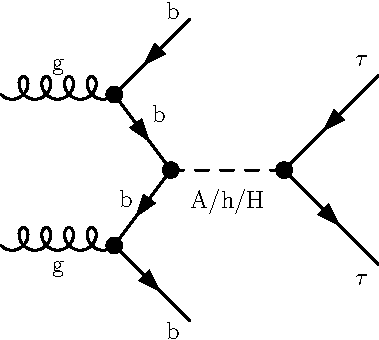
\includegraphics[height=3.5cm]{feyn_diagrams/diagrams/bbA.pdf}
     }\hspace{0.2cm}	
     \subfigure[]{		
            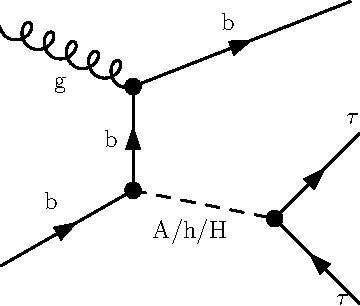
\includegraphics[height=3.5cm]{feyn_diagrams/diagrams/bbA2.pdf}
     }	\hspace{0.2cm}	
     \subfigure[]{		
            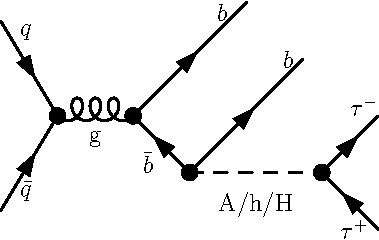
\includegraphics[height=3cm]{feyn_diagrams/diagrams/bbA3.pdf}
     }
     \subfigure[]{	
            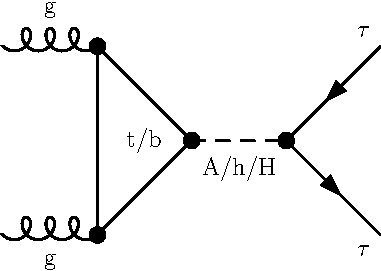
\includegraphics[height=3cm]{feyn_diagrams/diagrams/ggH.pdf}
	}	
     \end{center}
    \caption{Feynman diagram for the production of the neutral MSSM Higgs bosons in association with  $b$-quarks (a,b,c) and via gluon fusion (d) 
	processes, subsequent decay in tau lepton pairs is considered.}
   \label{fig:prod}
\end{figure}

\begin{figure}[tp]
     \begin{center}

     \subfigure[]{		
            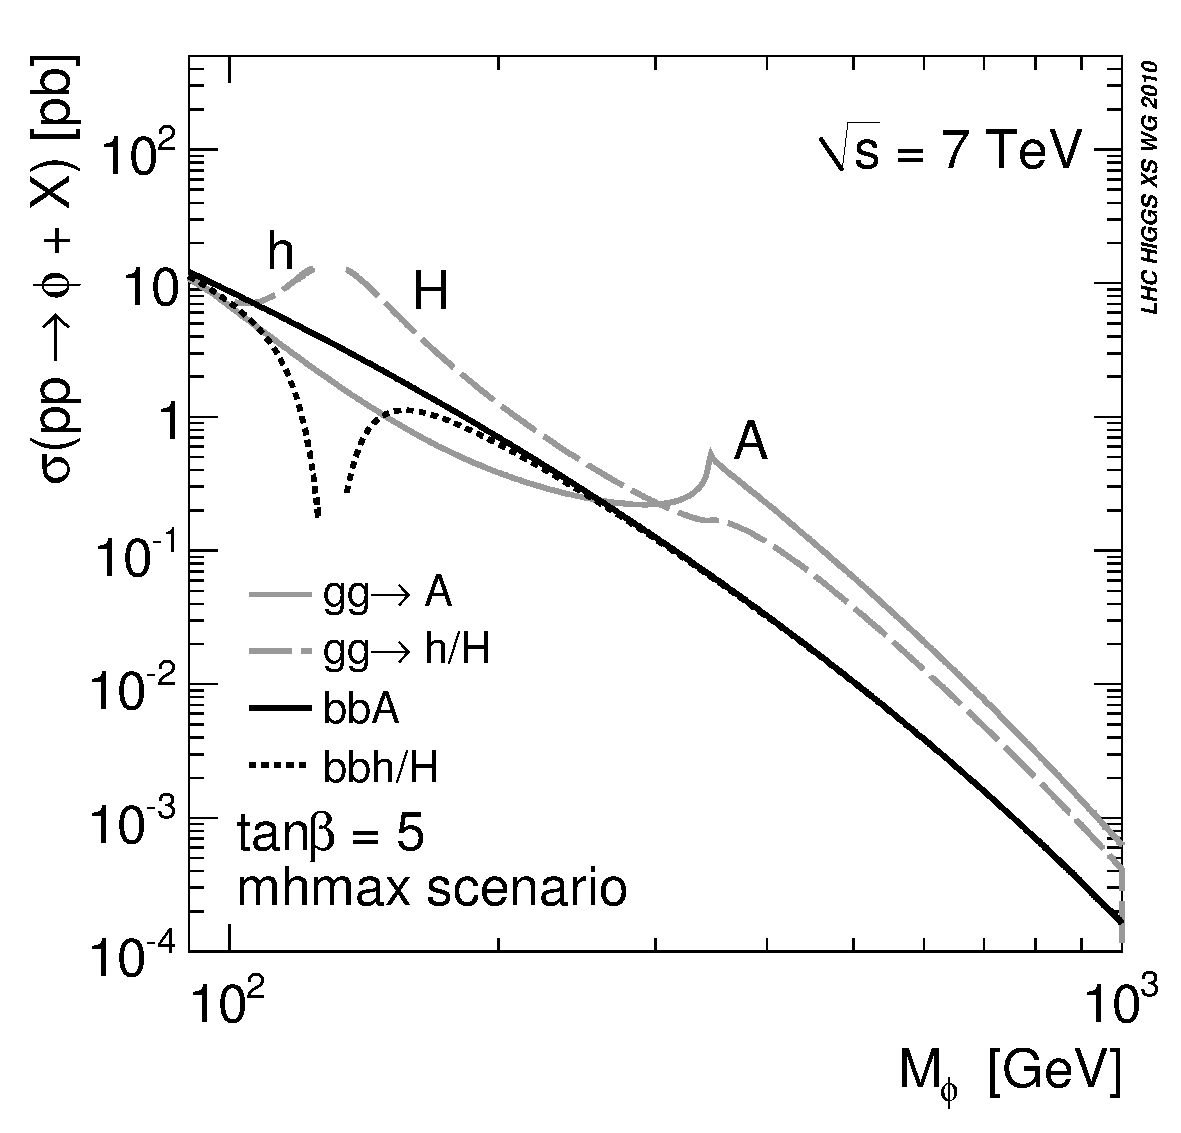
\includegraphics[width=0.6\textwidth]{figure/Xsec/YRHXS_MSSM_neutral_fig6a.pdf}
	}
     \subfigure[]{		
            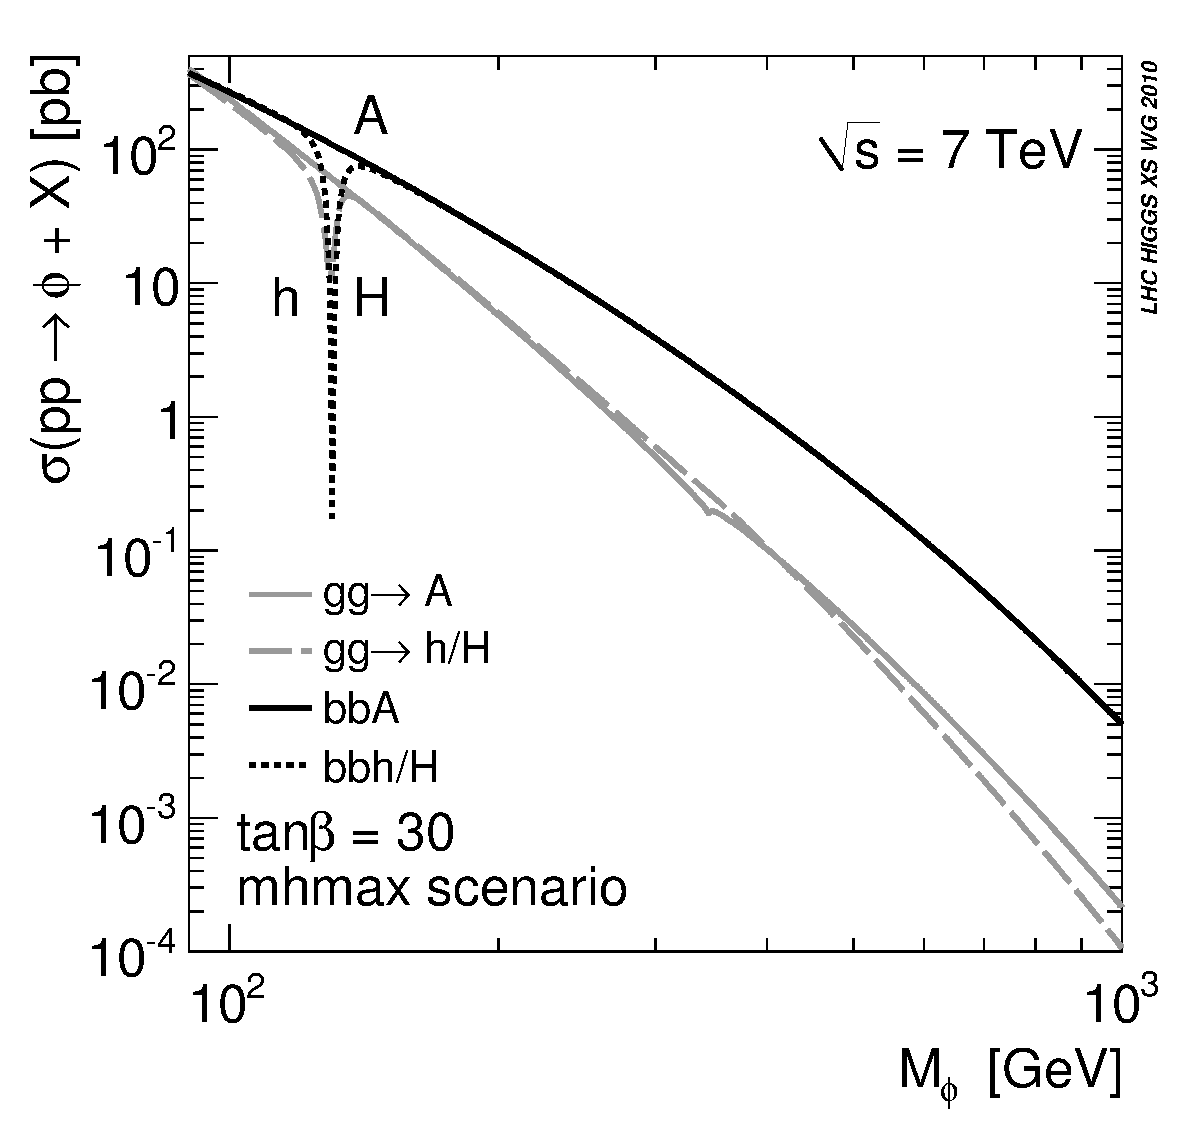
\includegraphics[width=0.6\textwidth]{figure/Xsec/YRHXS_MSSM_neutral_fig6b.pdf}
	}
    \end{center}
    \caption{Central predictions for the total MSSM Higgs bosons production cross sections via gluon fusion and Higgs radiation off
	bottom quarks  for $\sqrt{s} = 7$ TeV using NNLO and NLO MSTW2008 PDFs $m_h^{max}$ scenario; (a) $\tan\beta  = 5$, (b) $\tan\beta  = 30$.
	Reference~\cite{LHCxsec1}. }

   \label{fig:xsec}
\end{figure}


\begin{figure}[tp]
     \begin{center}

            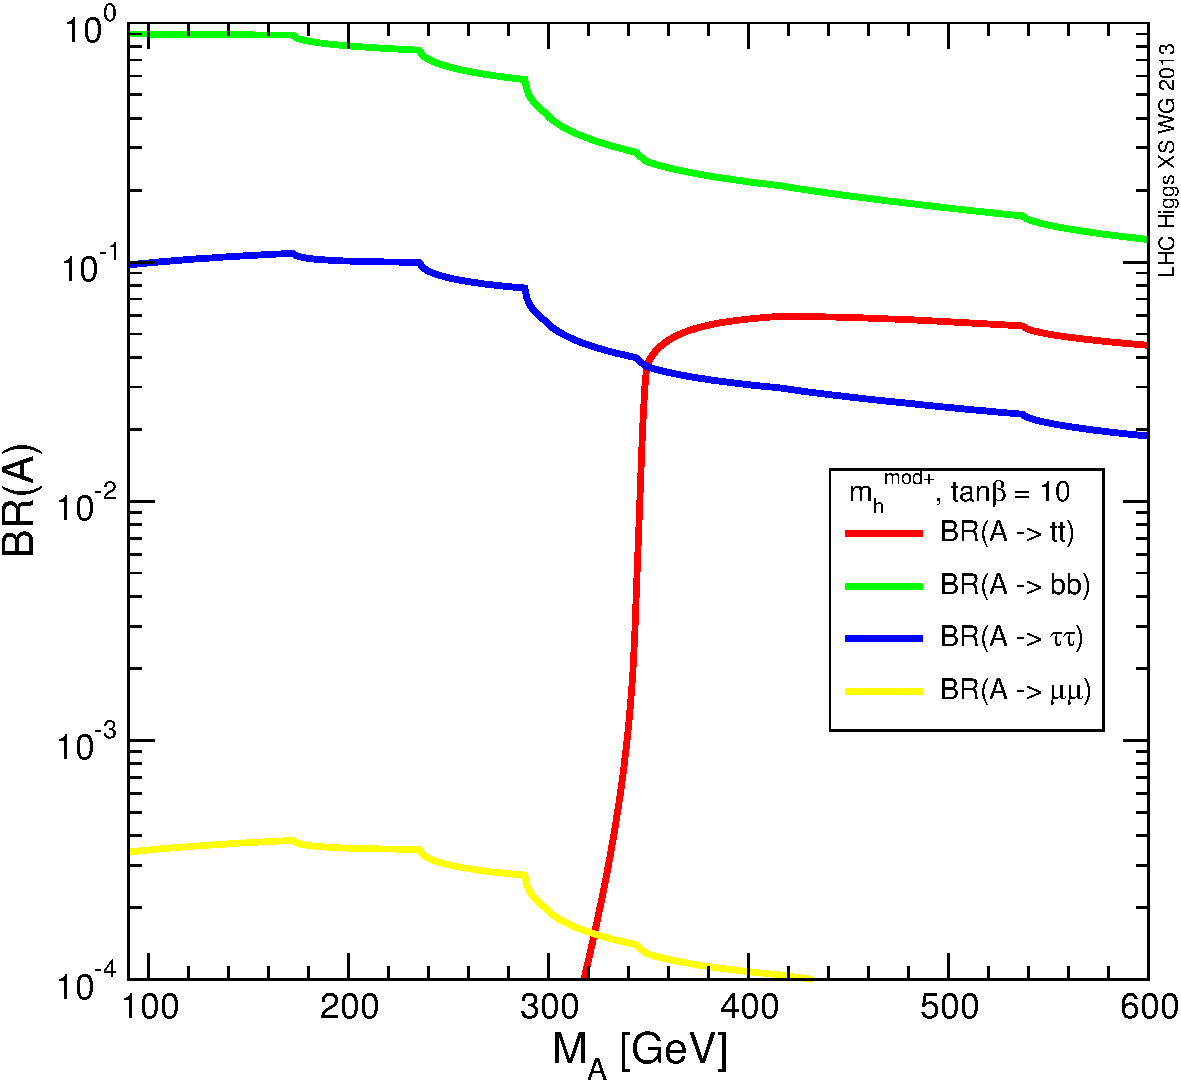
\includegraphics[width=0.47\textwidth]{figure/BR_higgs/YRHXS3_BR_fig31.pdf}
            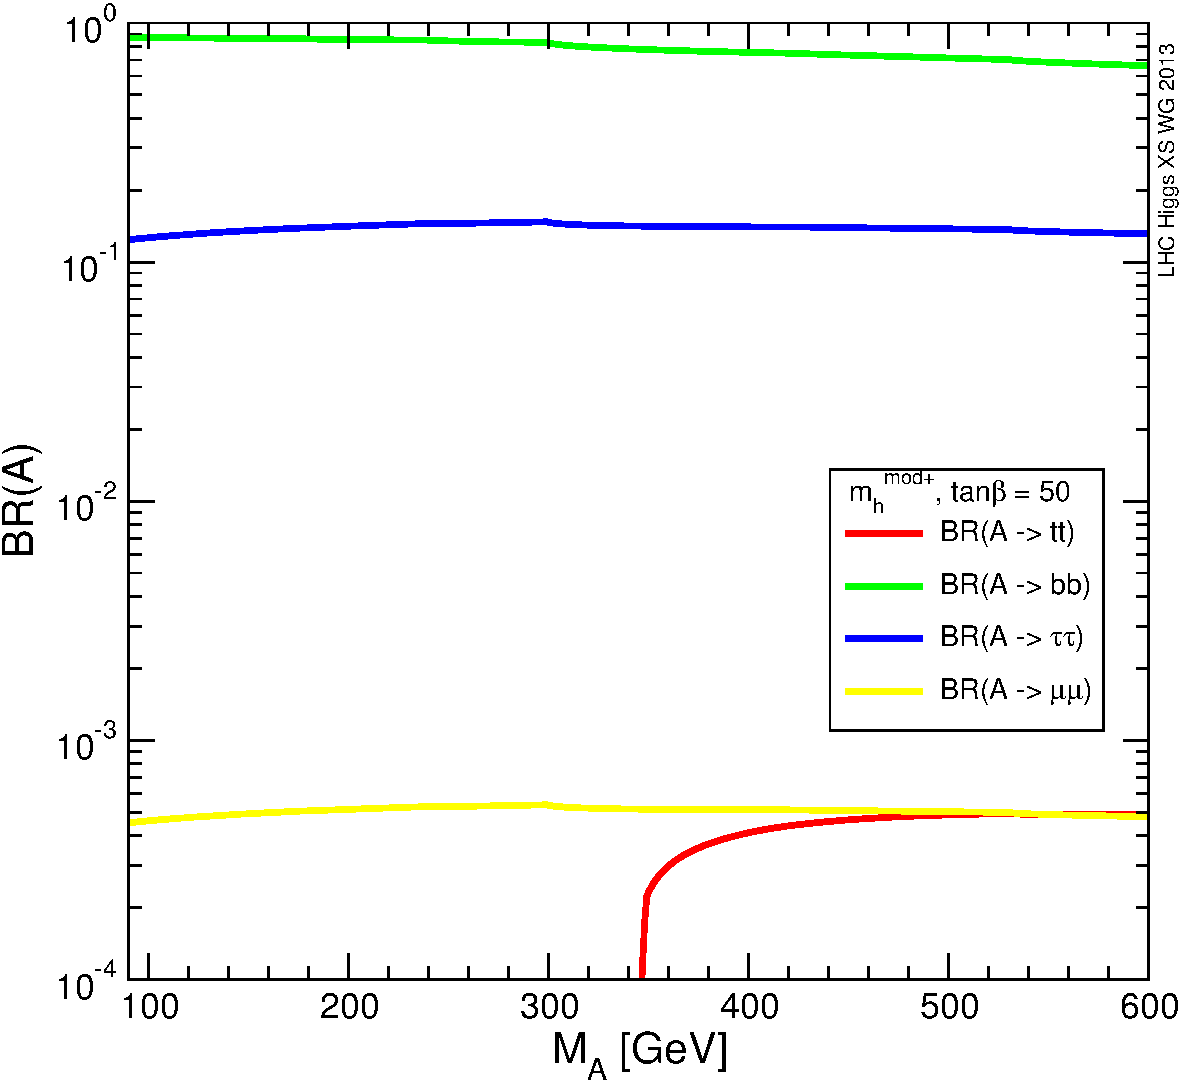
\includegraphics[width=0.47\textwidth]{figure/BR_higgs/YRHXS3_BR_fig32.pdf}
            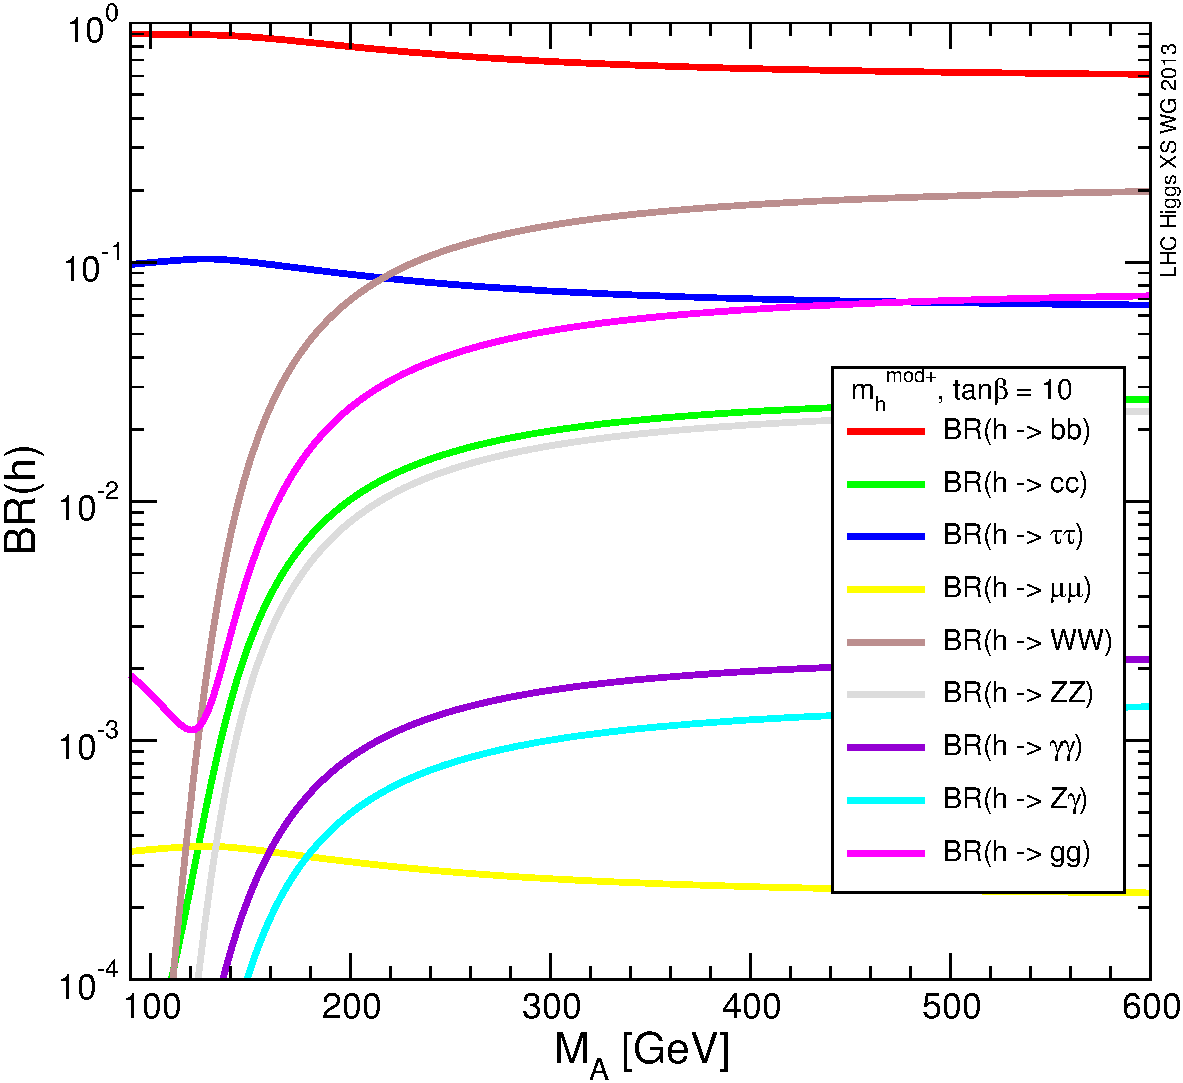
\includegraphics[width=0.47\textwidth]{figure/BR_higgs/YRHXS3_BR_fig35.pdf}
            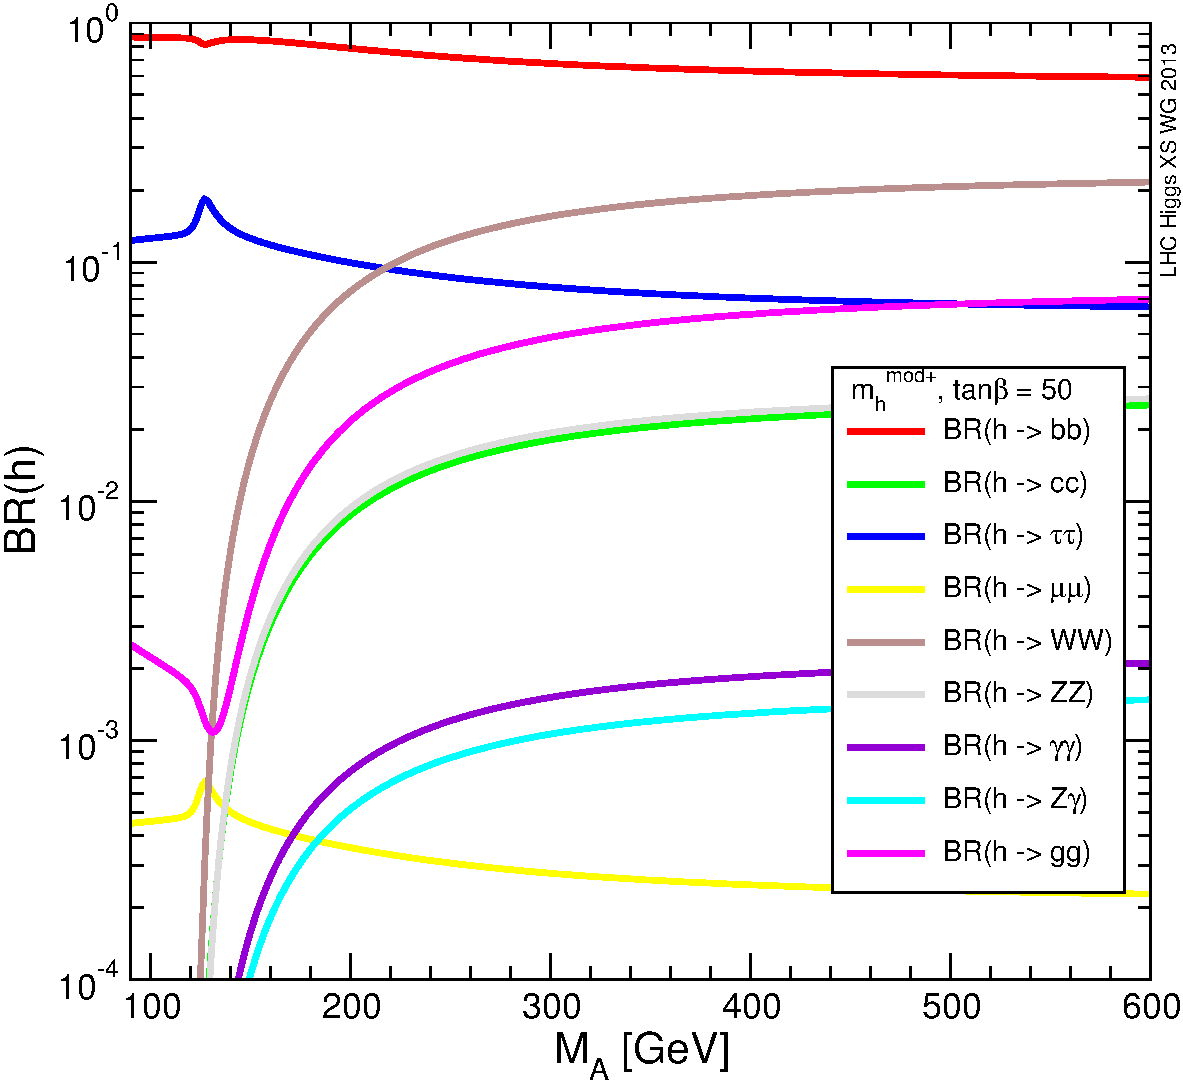
\includegraphics[width=0.47\textwidth]{figure/BR_higgs/YRHXS3_BR_fig36.pdf}
            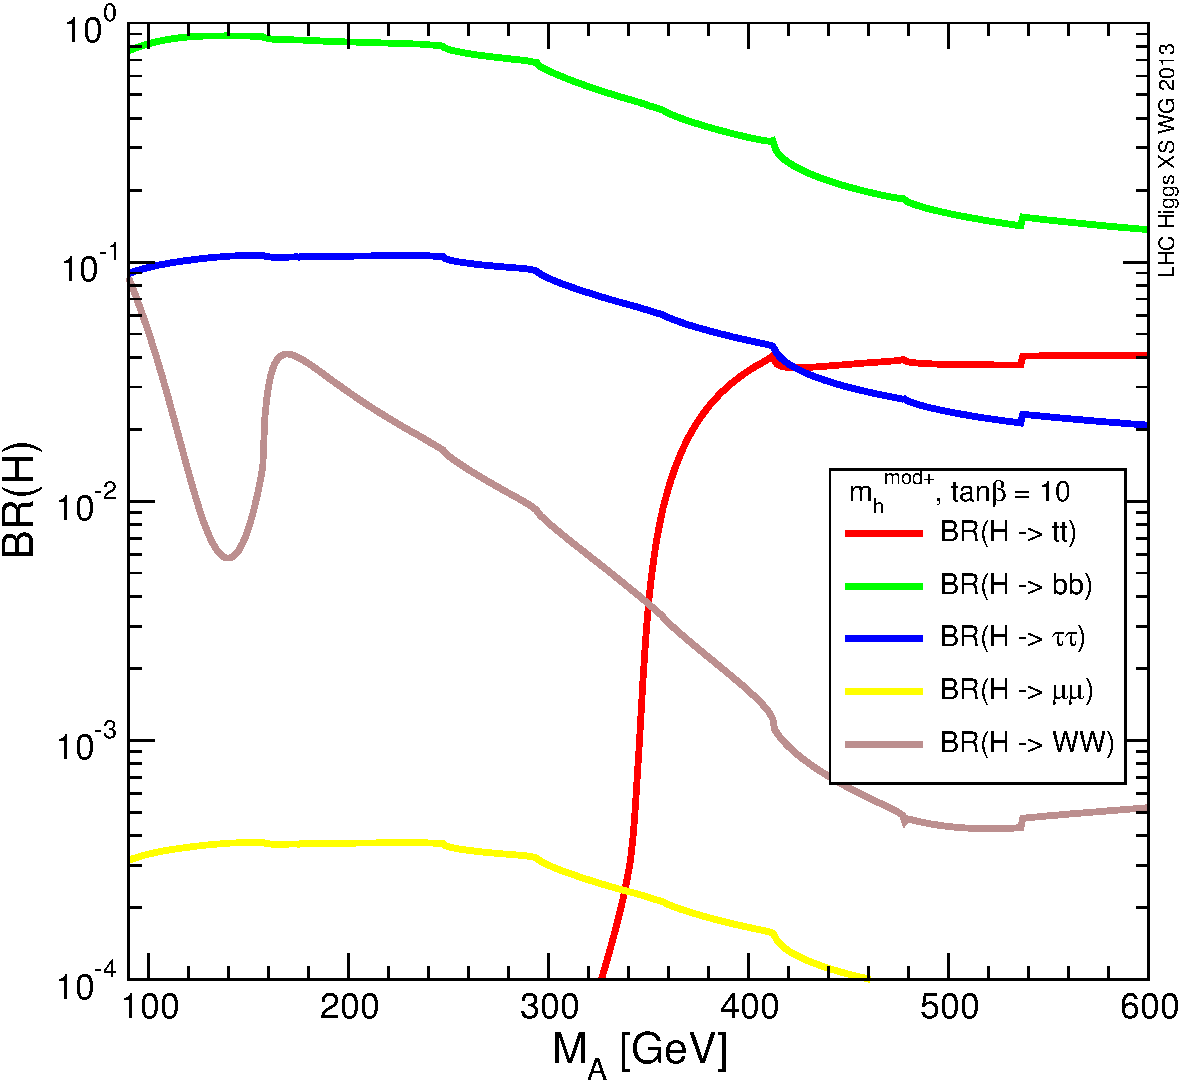
\includegraphics[width=0.47\textwidth]{figure/BR_higgs/YRHXS3_BR_fig37.pdf}
            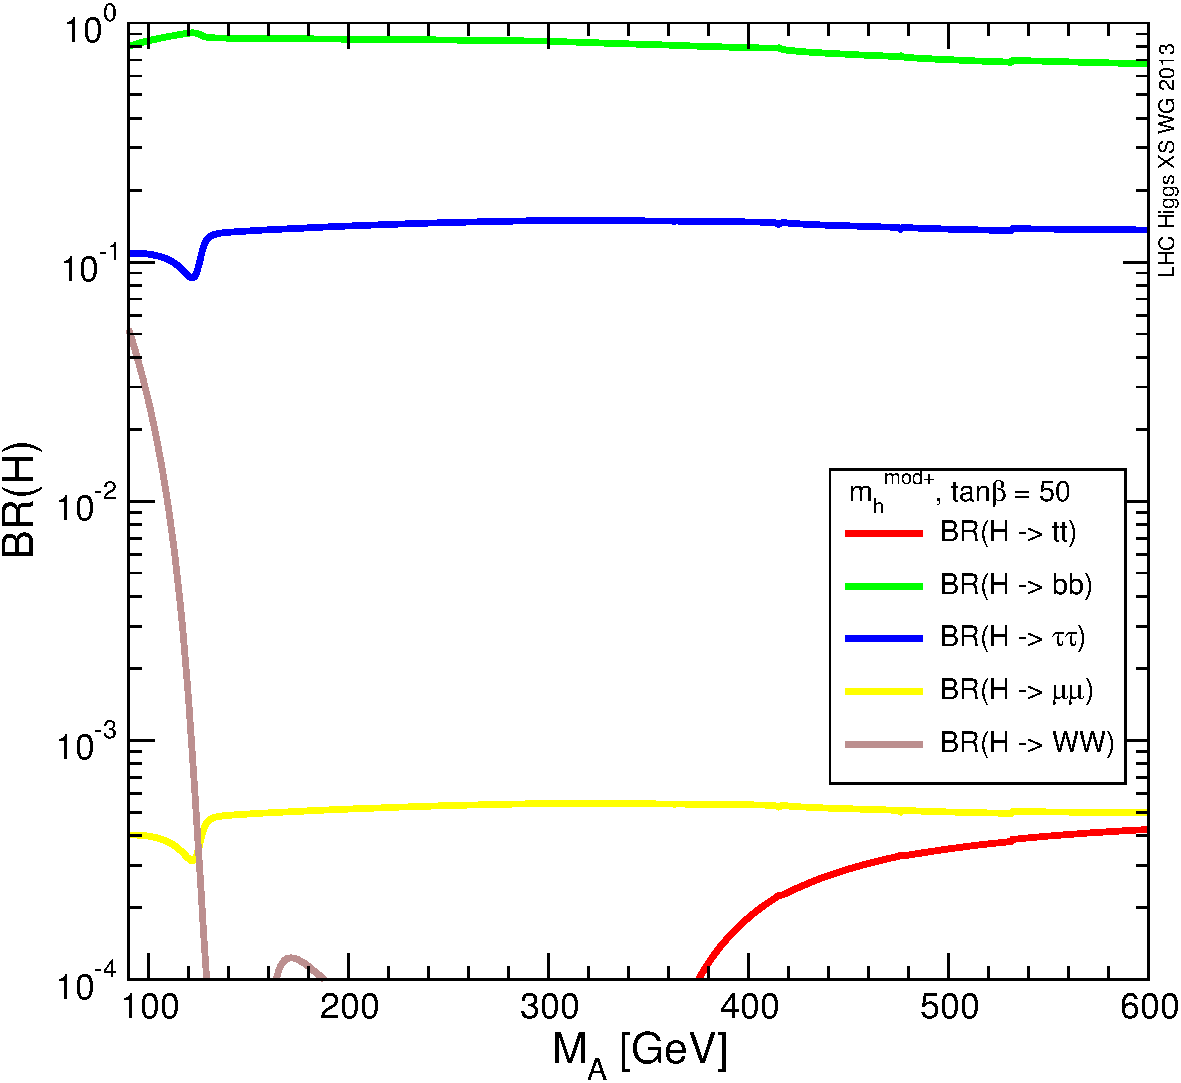
\includegraphics[width=0.47\textwidth]{figure/BR_higgs/YRHXS3_BR_fig38.pdf}

    \end{center}
    \caption{Branching fraction for the MSSM neutral Higgs bosons, $h/H/A$, in the $m_h^{mod+}$ scenario for $\tan\beta=10$ and
	$\tan\beta=50$. Reference~\cite{LHCxsec}.}
   \label{fig:br}

\end{figure}



\subsection{Current Status of the Search for Neutral MSSM Higgs Bosons}

The measure of the couplings of the observed SM-like Higgs boson can shed light on the Higgs sector and determine if this boson
is fully responsible for the generation of all the SM particles masses. 
%In fact, the couplings are sensitive to new physics,
%given the unitarity property of scattering amplitudes for longitudinal vectors and fermions, 
There are two approaches to explore the Higgs sector: one, is to use the measured Higgs couplings with SM particles to 
set constraint on new physics, while the other is to directly search for additional Higgs bosons in a well defined model.

In case the SM-like Higgs boson is interpreted as the light CP-even Higgs boson of the MSSM, the couplings of the Higgs boson 
to vector bosons ($k_V$), up-type fermions ($k_u$) and down-type fermions ($k_d$), can be expressed as a function of  $m_A $ and $\tan\beta$ 
and this allow to set exclusion limits in the $m_A - \tan\beta$ plane~\cite{AtlasConstraint}. Figure~\ref{fig:ex1} shows the exclusion limits in a 
``simplified MSSM'' model~\cite{sympleMSSM1,sympleMSSM2} via fits to the measured rates of Higgs boson production and decay.

 
\begin{figure}[tp]
     \begin{center}

            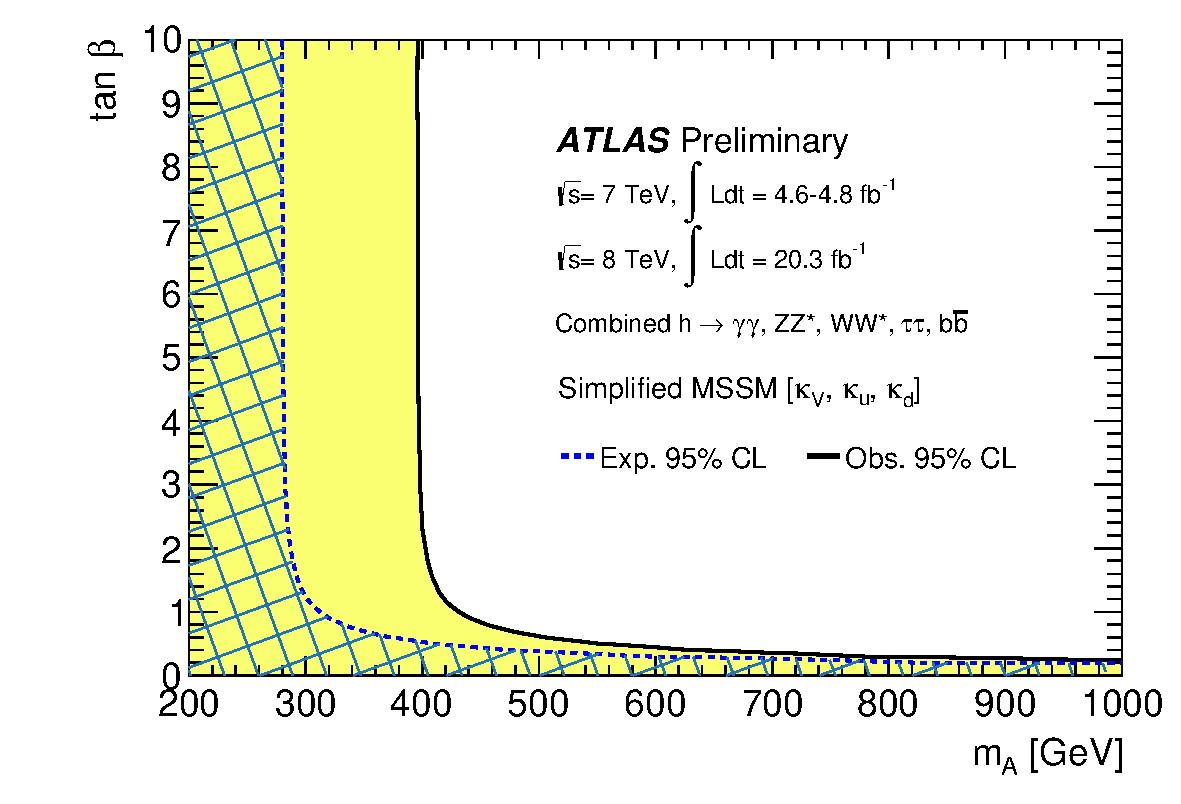
\includegraphics[width=0.8\textwidth]{figure/limits/constraintAtlas.pdf}

    \end{center}
    \caption{Regions of the  $m_A - \tan\beta$ plane excluded in a simplified MSSM model via fits to the measured
rates of Higgs boson production and decays. The likelihood contours where $−2 \ln \Lambda = 6.0$, corresponding
approximately to 95\% CL ($2\sigma$), are indicated for the data and expectation assuming the SM Higgs sector.
The light shaded and hashed regions indicate the observed and expected exclusions, respectively. The
SM decoupling limit is $m_A \rightarrow \infty$. See Reference~\cite{AtlasConstraint}.}

   \label{fig:ex1}
\end{figure}


The current latest constraint on $m_A - \tan\beta$  by direct search of neutral MSSM Higgs bosons~\cite{} are  shown in Figure~\ref{fig:ex2}
and are part of the work of this thesis.



 
\begin{figure}[tp]
     \begin{center}

            
\includegraphics[width=0.8\textwidth]{figure/blank.pdf}

    \end{center}
    \caption{Limit CMS or ATLAS depending if we manage to publish in time}


   \label{fig:ex2}
\end{figure}




















